\chapter{Sistemi dinamici interconnessi}
	
\section{Schemi a blocchi}
	\figura{5.5}{1}{sist-int}{esempio di sistema dinamico interconnesso.}{sist-int}
	
	\begin{concetto}
		L'\textbf{analisi di sistemi dinamici interconnessi} permette di studiare come una concatenazione (eventualmente retro-azionata) di sistemi si comporta rispetto all'analisi dei sistemi singoli. Questa analisi viene effettuata generalmente tramite il formalismo degli \textbf{schemi a blocchi} (i cui elementi costitutivi sono descritti in figura \ref{fig:int:elementicostitutivi}) che semplifica e rende sistematico il processo di analisi.
	\end{concetto}
	
	In particolare il \textbf{blocco} è la \textit{black box} che rappresenta il sistema dinamico: esso contiene dunque dei rami in ingresso ($U$ in figura \ref{fig:int:elementicostitutivi}.a), eventualmente multipli, che tramite una funzione di trasferimento $G(s)$ determinano un'uscita $Y$ (nel dominio di Laplace) secondo la cosiddetta \textbf{\textit{equazione costitutiva}}
	\[  Y(s) = G(s) U(s) \]
	Il \textbf{nodo sommatore} (figura \ref{fig:int:elementicostitutivi}.b) permette, come suggerisce il nome, di sommare (o sottrarre) una serie di rami provenienti dall'esterno o da un'altro blocco; la \textbf{diramazione} (figura \ref{fig:int:elementicostitutivi}.c) invece permette di creare un valore multiplo di rami (che condividono lo stesso valore) a partire da un'unico ramo.
	
	\begin{figure}[bht]
		\centering
		\begin{subfigure}{0.325\linewidth}
			\centering 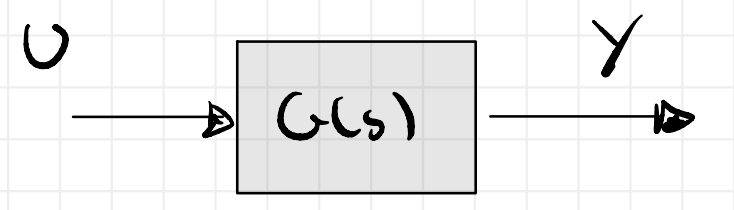
\includegraphics[width=4cm]{blocco} \caption{}
		\end{subfigure}
		\begin{subfigure}{0.325\linewidth}
			\centering 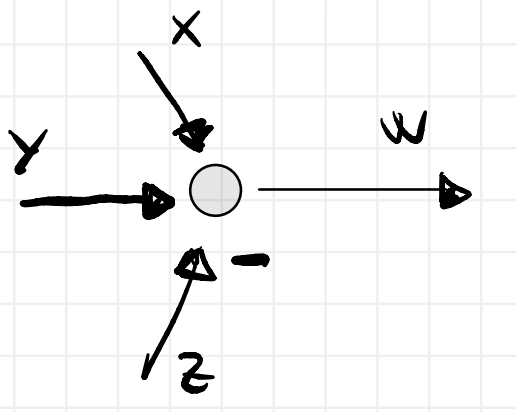
\includegraphics[width=2.5cm]{sommatore} \caption{}
		\end{subfigure}
		\begin{subfigure}{0.325\linewidth}
			\centering 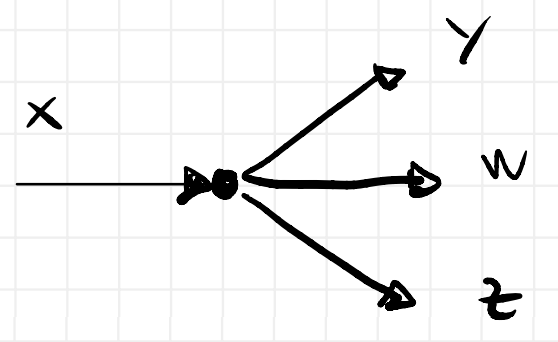
\includegraphics[width=2.5cm]{diramazione} \caption{}
		\end{subfigure}
		\caption{rappresentazione grafica degli elementi costitutivi della rappresentazione mediante schemi a blocchi: il blocco (a), il nodo sommatore (b) e la diramazione (c).}
		\label{fig:int:elementicostitutivi}
	\end{figure}
	
	Anche per il sommatore e la diramazione è possibile creare delle equazioni caratteristiche associate; considerando il sommatore nel disegno di esempio è possibile infatti affermare che 
	\[ w = x + y -z \]
	mentre alla diramazione è associata un sistema di equazioni del tipo $y=x$, $w = x$ e $z = x$.
	
	\subsection{Connessioni elementari}
		
		\begin{concetto}
			Nella rappresentazione mediante schemi a blocchi i vari sistemi dinamici possono essere collegati in modo \textit{svariato}, tuttavia ogni situazione può essere scomposta in livelli \textit{elementari} arrivando a determinare 3 tipi di \textbf{connessioni elementari} tra circuiti (figura \ref{fig:int:connesioni-elementari}): \textbf{collegamento in serie}, in \textbf{parallelo} e in \textbf{retroazione}. In particolare la funzione di trasferimento associata ad ogni connessione, per come verrà dimostrato, vale
			\begin{equation}
				G_\textrm{serie} =  \prod_i G_i \qquad G_\textrm{parallelo} = \sum_i G_i \qquad G_\textrm{feedback} = \frac{G_1}{1\mp G_1G_2}
			\end{equation}
		\end{concetto}
	
		\begin{figure}[bht]
			\centering
			\begin{subfigure}{0.325\linewidth}
				\centering 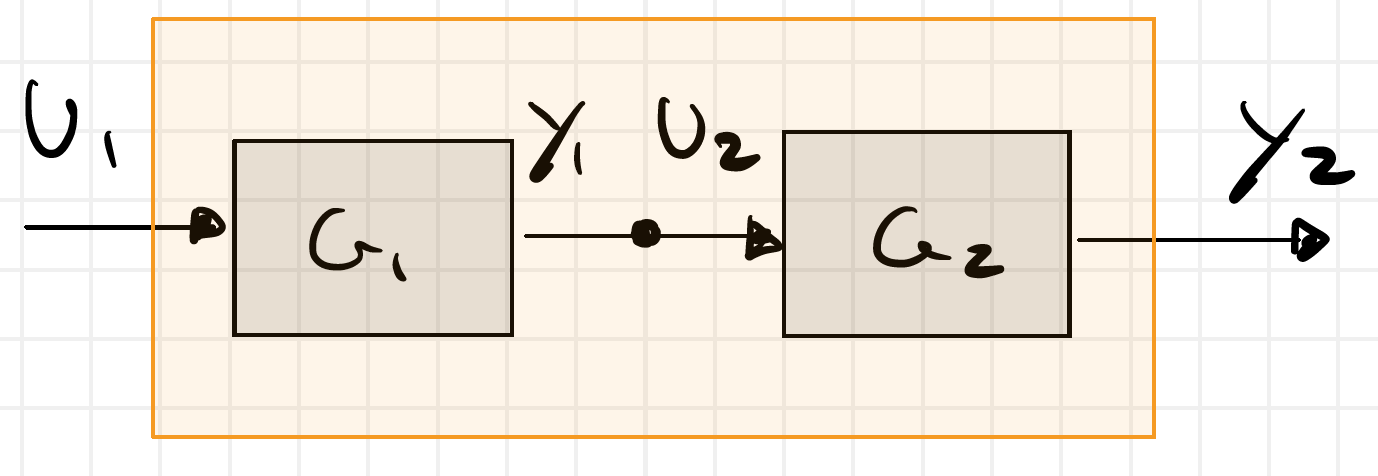
\includegraphics[width=4cm]{serie} \caption{}
			\end{subfigure}
			\begin{subfigure}{0.325\linewidth}
				\centering 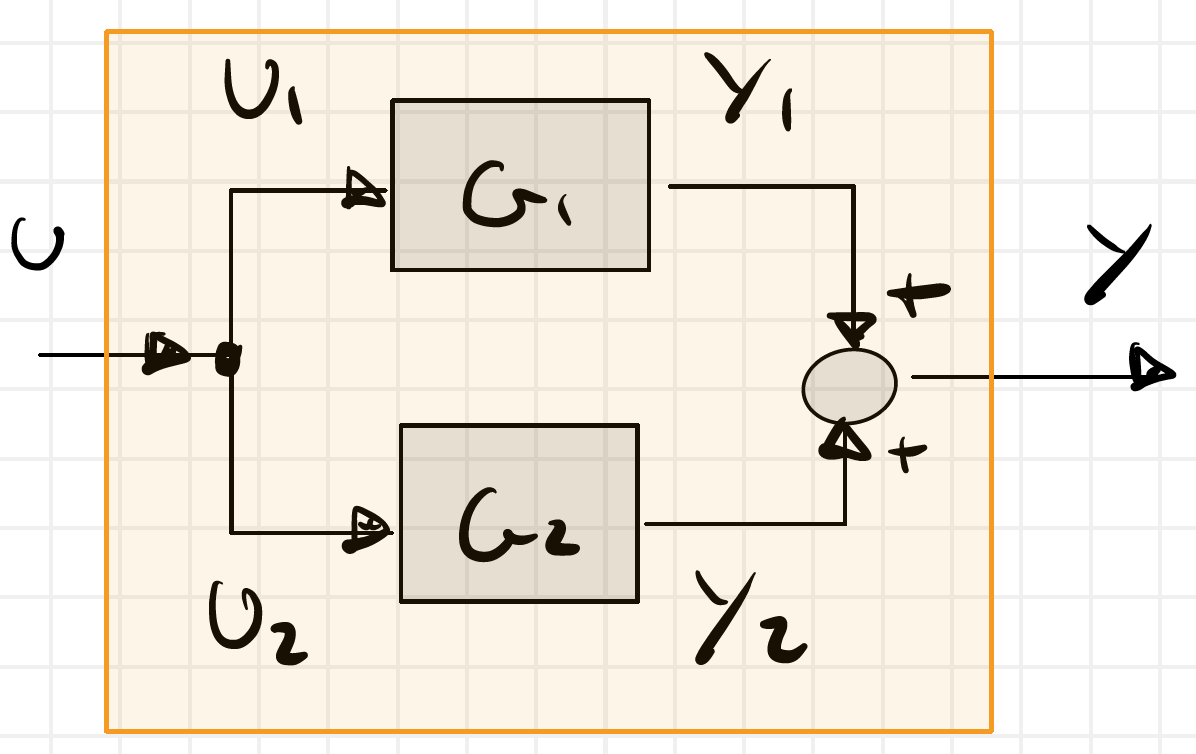
\includegraphics[width=3.5cm]{parallelo} \caption{}
			\end{subfigure}
			\begin{subfigure}{0.325\linewidth}
				\centering 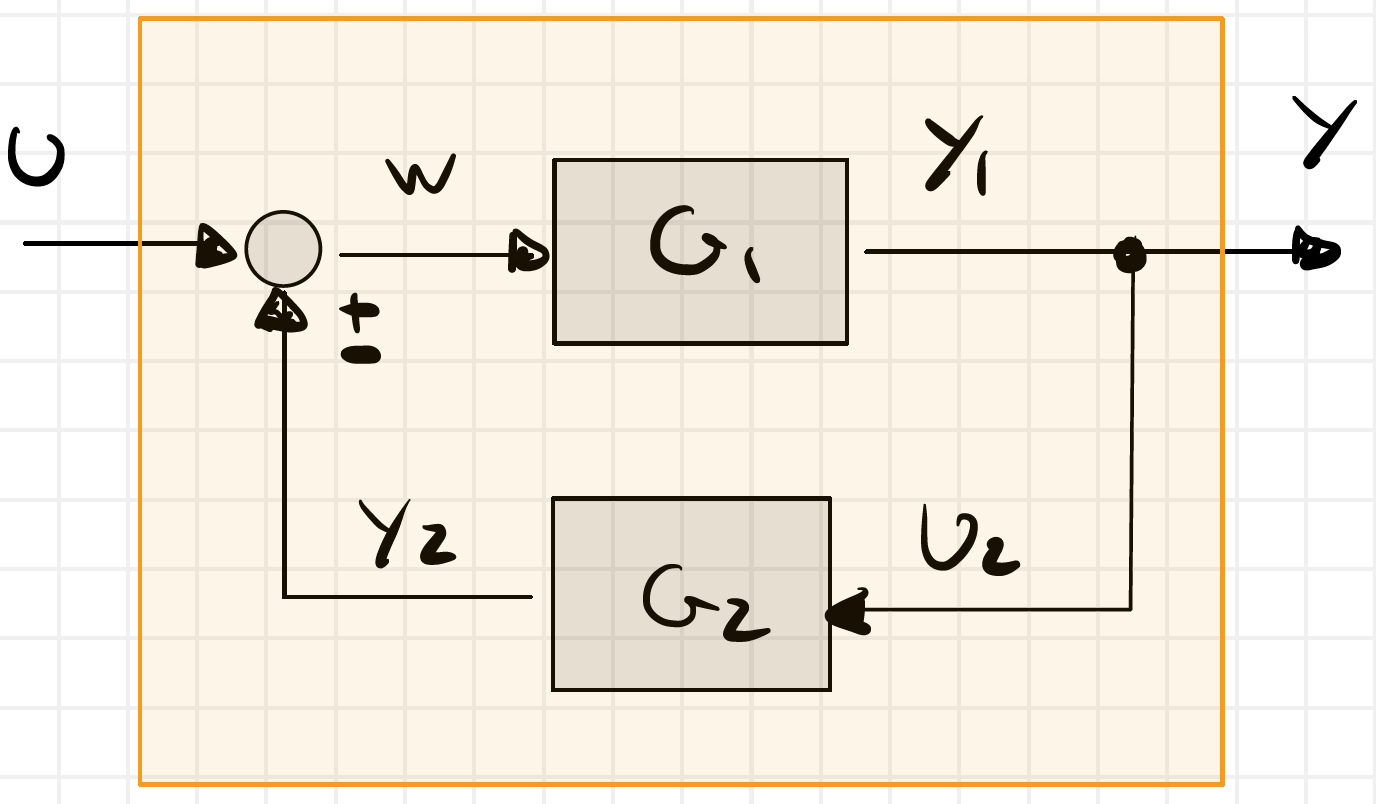
\includegraphics[width=4.5cm]{retroazione} \caption{}
			\end{subfigure}
			\caption{rappresentazione tramite schema a blocchi delle connessioni elementari che è possibile individuare negli schemi: connessione in serie (a), in parallelo (b) e in retroazione (c).}
			\label{fig:int:connesioni-elementari}
		\end{figure}
		
		Partendo dall'analisi della connessione in \textbf{serie}, è possibile osservare che l'uscita $Y_1$ del primo sistema (ottenuta come $G_1U_1$) coincide con l'ingresso del secondo sistema: esplicitando dunque le equazioni che governano lo schema a blocchi si arriva a determinare
		\[ \begin{cases}
			Y_1 =G_1U_1 \\
			Y_2 =G_2U_2 \\
			U_2 = Y_1 \\ Y =Y_2 \\ U=U_1 
		\end{cases} \qquad Y_2 = G_2G_1U_1 \qquad \Rightarrow \quad G_\textrm{serie} = G_2G_1 \]
		
		In maniera analoga si può dimostrare la funzione di trasferimento $G$ associata ad una connessione in \textbf{parallelo}: noto infatti che l'ingresso $U_1,U_2$ dei due sistemi è uguale e pari ad $U$, mentre la loro uscita viene sommata da un nodo sommatore, allora
		\[ Y = Y_1+Y_2 = G_1U+G_2U \qquad \Rightarrow\qquad G_\textrm{parallelo} = G_1+G_2 \]
		
		Più complesso è analizzare un sistema in \textbf{retroazione}, tuttavia esplicitando tutte le relazioni si determina che
		\[G_\textrm{feedback} = \frac{G_1}{1\mp G_1G_2}  \]
		In maniera generale a numeratore della trasformata razionale è necessario scrivere la funzione di trasferimento della linea di mandata (ossia quella che collega direttamente ingresso e uscita), mentre al denominatore è necessario inserire la \textbf{funzione d'anello} $L(s)$, determinata dal guadagno che si ottiene percorrendo un giro dell'anello di retroazione:
		\[  G_\textrm{feedback} = \frac{G \textrm{ linea di mandata}}{1 \mp \textrm{funzione d'anello}} \]
		Si osserva che se l'uscita viene retro-azionata negativamente (ossia viene sottratta all'ingresso) è necessario utilizzare l'espressione di $G_f(s)$ con segno positivo a denominatore, mentre se la retro-azione è positiva allora si deve sottrarre a 1 la funzione $L(s)$.
		
		\begin{esempio}{: calcolo del guadagno d'anello}
			Si consideri lo schema a blocchi in figura:
			\begin{center}
				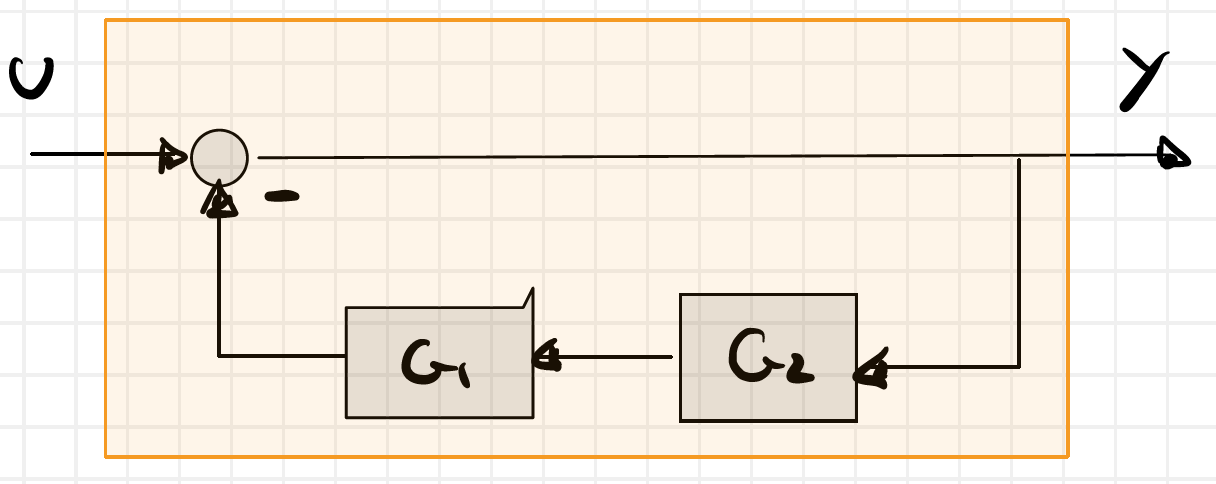
\includegraphics[width=5cm]{retroazione-b}
			\end{center}
			Osservando che nella linea di mandata non si ha la presenza di alcun blocco, allora il guadagno complessivo della linea sarà unitario. Analizzando invece l'anello si osserva che esso è costituito dalla serie tra $G_1$ e $G_2$, e dunque sfruttando tale connessione elementare deve valere $L = G_1G_2$. Essendo la retroazione negativa allora si può scrivere la funzione di trasferimento del sistema retro-azionato come
			\[ G_f = \frac 1 {1+G_1G_2} \]
		
		\end{esempio}
	
	\subsection{Rappresentazione dei sistemi dinamici}
		Fino ad ora nella trattazione della rappresentazione di sistemi a blocchi si è fatto riferimento, a livello intuitivo, a sistemi di tipo SISO, dove ad ogni \textit{scatola} che rappresenta un sistema si ha in ingresso una sola entrata e dalla quale esce una sola uscita. 
		\begin{concetto}
			Considerando in realtà i sistemi reali è possibile osservare che negli stessi esistono svariati tipi di \textbf{ingressi} che oltre a quelli \textbf{propri} (denotati generalmente $u$), possono essere di \textbf{disturbo} $d$ (come in figura \ref{fig:int:disturbo} o di \textbf{rumore} $n$.
		\end{concetto}
		\begin{nota}
			Si parla in particolare di ingressi di disturbo quando essi influenzano la funzione di trasferimento $G(s)$ di un sistema dinamico, mentre si parla di rumore quando il valore dell'ingresso va a sommarsi ad una diramazione.
		\end{nota}
		
		\begin{figure}[bht]
			\centering
			\begin{subfigure}{0.48\linewidth}
				\centering 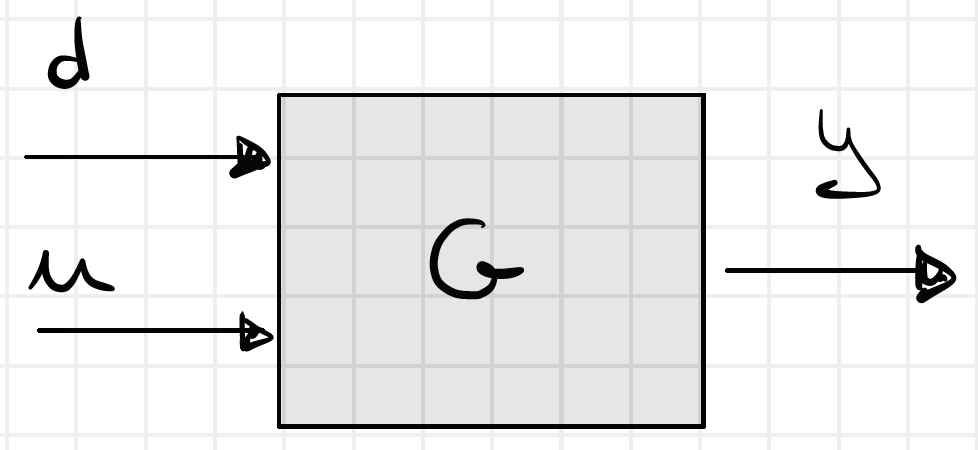
\includegraphics[width=4cm]{dist-a} \caption{}
			\end{subfigure}
			\begin{subfigure}{0.48\linewidth}
				\centering 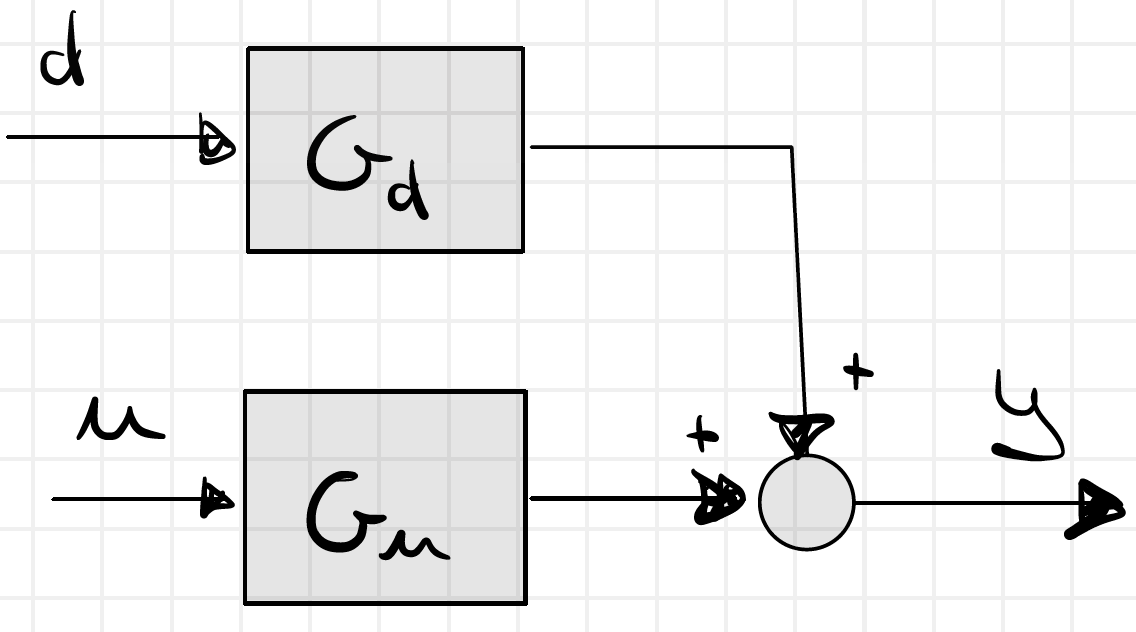
\includegraphics[width=4cm]{dist-b} \caption{}
			\end{subfigure}
			\caption{rappresentazione "semplificata" (a) ed "estesa" (b) di un sistema dinamico la cui uscita dipende sia dall'ingresso proprio $u$ che dall'ingresso di disturbo $d$.}
			\label{fig:int:disturbo}
		\end{figure} 
		
		\begin{concetto}
			I \textbf{sistemi di controllo}, per come già visto a pagina \pageref{sec:sistemacontrollo}, sono dunque caratterizzati dal collegamento due sistemi dinamici (in generale il collegamento è in retroazione negativa in quanto permette di determinare delle prestazioni \textit{migliori}): il \textbf{regolatore} con funzione di trasferimento $R$ e il sistema $G$. \\
			In particolare come \textbf{ingresso} al sistema si osserva il \textbf{valore di riferimento} $\overline y$ al quale dovrebbe tendere l'uscita e gli ingressi di disturbo $d$ e di rumore $n$; in \textbf{uscita} invece è possibile rilevare sia l'uscita $y$ che l'errore $e$ (differenza tra $\overline y$ e $y$) e la variabile controllata $u$.
			\begin{center}
				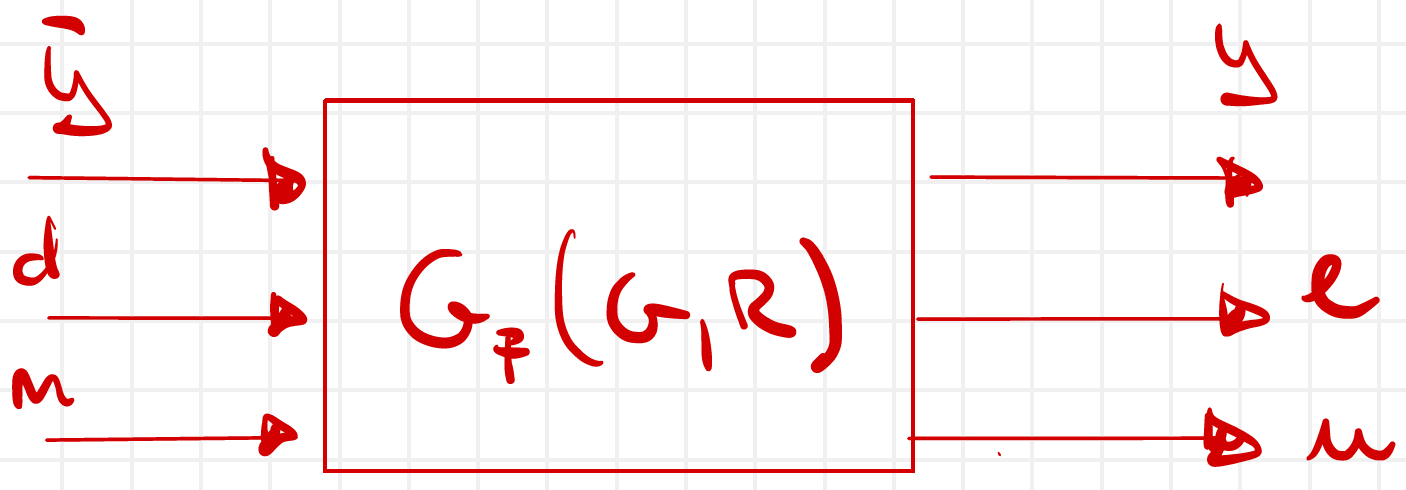
\includegraphics[width=4cm]{intercon-a}
			\end{center}
		\end{concetto}
		
		\begin{figure}[bht]
			\centering
			\begin{subfigure}{0.325\linewidth}
				\centering 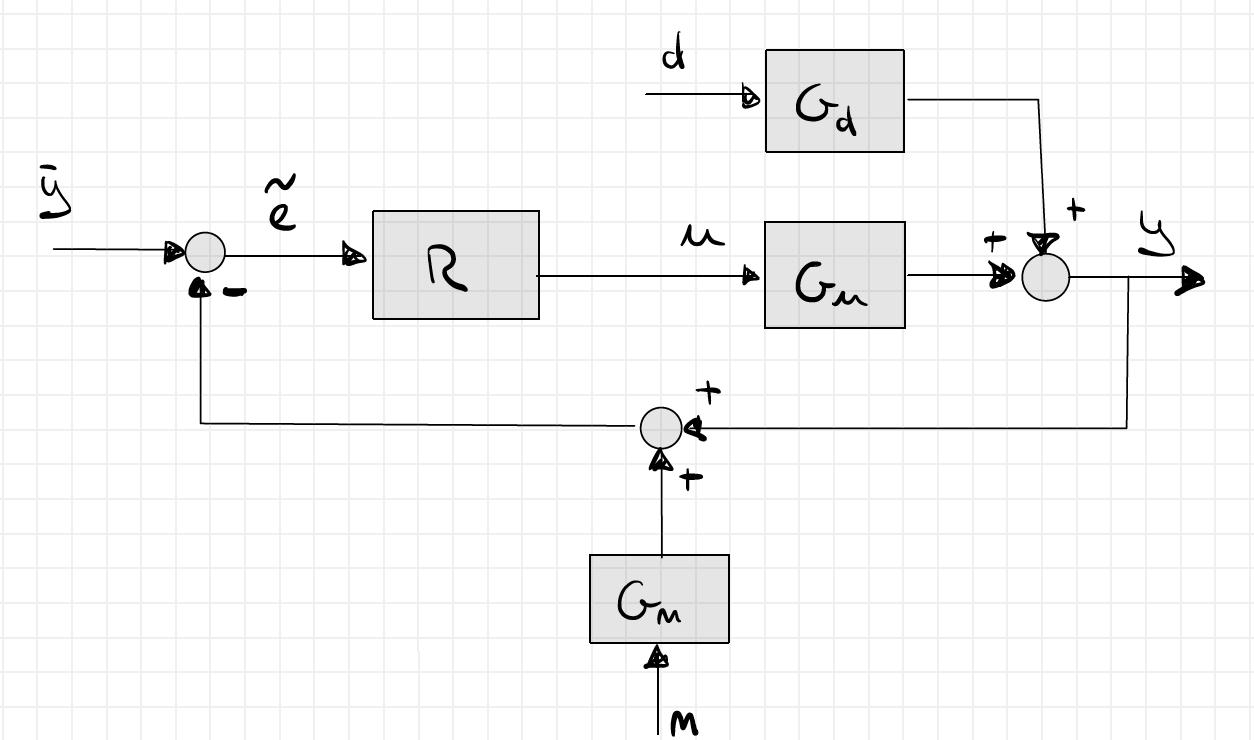
\includegraphics[width=0.98\linewidth]{intercon-b} \caption{}
			\end{subfigure}
			\begin{subfigure}{0.325\linewidth}
				\centering 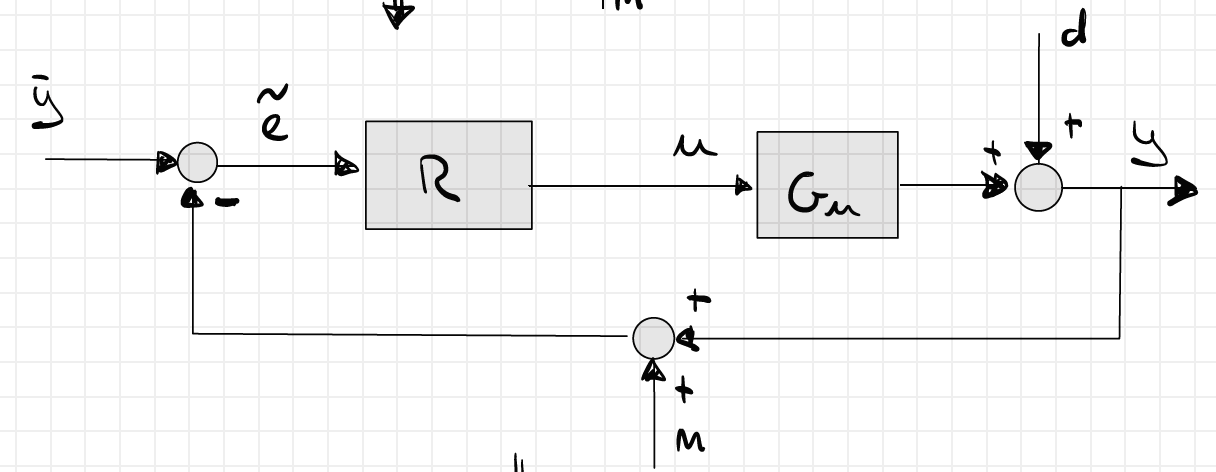
\includegraphics[width=0.98\linewidth]{intercon-c} \caption{}
			\end{subfigure}
			\begin{subfigure}{0.325\linewidth}
				\centering 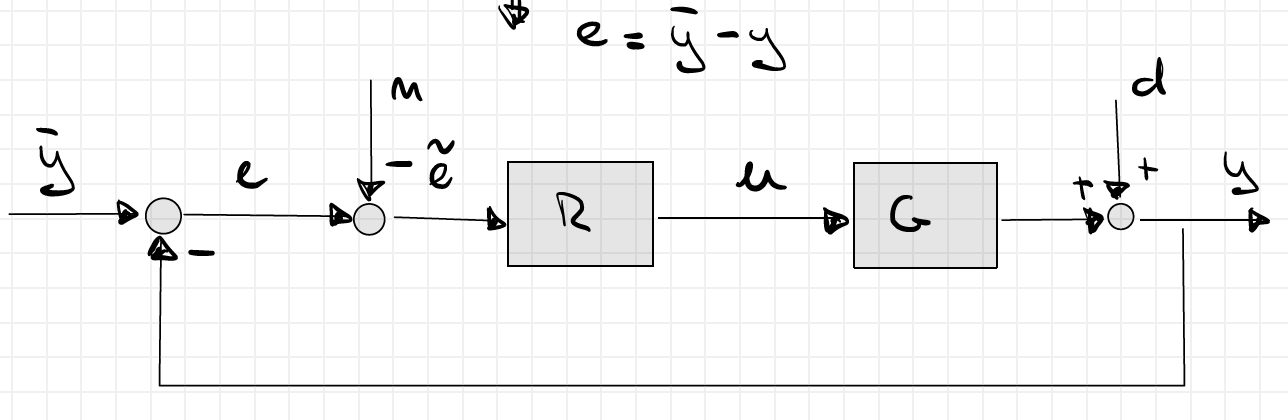
\includegraphics[width=0.98\linewidth]{intercon-d} \caption{}
			\end{subfigure}
			\caption{diverse rappresentazioni generali di un sistema in retroazione negativa.}
			\label{fig:int:rappsimili}
		\end{figure}
		
\section{Stabilità di sistemi interconnessi}
	Lo studio della stabilità di sistemi interconnessi è fondamentale, in quanto si vuole capire \textit{quando} (ma soprattutto \textit{in che modo}) è possibile controllare ottimalmente un sistema di controllo, in particolare per che tipo di regolatore e la sua connessione con il sistema è possibile ottenere dei risultati \textit{buoni} (in particolar modo se è possibile stabilizzare un sistema che, considerato singolarmente, sarebbe instabile).
	
	Considerando la connessione in serie e parallelo di due sistemi la cui funzione di trasferimento razionale $G_i$ è espressa dai rapporti $N_i/D_i$, allora esplicitando la funzione di trasferimento complessiva si ottiene
	\[ G_\textrm{serie} =G_1G_2 = \frac{N_1}{D_1} \frac{N_2}{D_2} = \frac N D \qquad G_\textrm{parallelo} = G_1 + G_2 = \frac{N_1}{D_1}+ \frac{N_2}{D_2} = \frac{N_1D_2 + N_2D_1}{D_1D_2} = \frac N D  \]
	
	\begin{concetto}
		La \textbf{connessione in serie/parallelo} di due sistemi con funzione di trasferimento razionale determina una \textbf{funzione di trasferimento} complessiva che risulterà anch'essa essere \textbf{razionale} la cui particolarità è che il denominatore $D$ coincide con la moltiplicazione dei denominatori $D_1,D_2$ dei blocchi che compongono la connessione.
		
		Questo significa dunque \textbf{\textit{unire i poli}} delle funzioni $G_1,G_2$: se dunque anche solo uno dei due sistemi è instabile, allora anche il sistema risultante sarà instabile.
	\end{concetto}
	Tramite una connessione in serie/parallelo non è mai possibile stabilizzare un sistema che in origine è instabile.
	
	Osservato che la connessioni appena descritte sono tendenzialmente inefficaci a stabilizzare i sistemi (che nella pratica spesso sono instabili), allora è possibile analizzare la connessione in retroazione; esplicitando le funzioni di trasferimento si osserva che
	\[ G_\textrm{feedback} = \frac{ G_1}{ 1 \mp G_1G_2} = \frac{N_1/D_1}{1\mp \dfrac{N_1}{D_1}\dfrac{N_2}{D_2}} = \frac{N_1D_2}{D_1D_2 \mp N_1N_1} = \frac N D \]
	Anche in questo caso la trasformata complessiva del sistema retroazionato risulta essere razionale, tuttavia va notato che, a differenza della connessione in serie/parallelo, il denominatore di $G_f$ cui sono associati i suoi poli non dipende solamente dal denominatore di $G_1,G_2$, ma anche dal numeratore. In generale dunque i poli di $G_f$ sono differenti da quelli dei sistemi di origine $G_1,G_2$.
	
	Questo significa che se il collegamento di due sistemi asintoticamente stabili può non portare ad un sistema asintoticamente stabile, come analogamente se un sistema è instabile non è detto che il sistema retroazionato sia instabile. \\
	In generale se un sistema è instabile, esso può essere stabilizzato tramite un collegamento in retroazione con un opportuno sistema dinamico.
		
	\begin{concetto}
		La \textbf{stabilità} di un \textbf{sistema retroazionato} si dimostra essere dipendente solamente dalle proprietà della funzione d'anello $L(s)$, e non dalla posizione relativa dei blocchi (che dunque possono essere posti indifferentemente sia sulla linea di mandata, che di feedback). Per esempio i seguenti sistemi, ai fini della stabilità, sono equivalenti:
		\begin{center}
			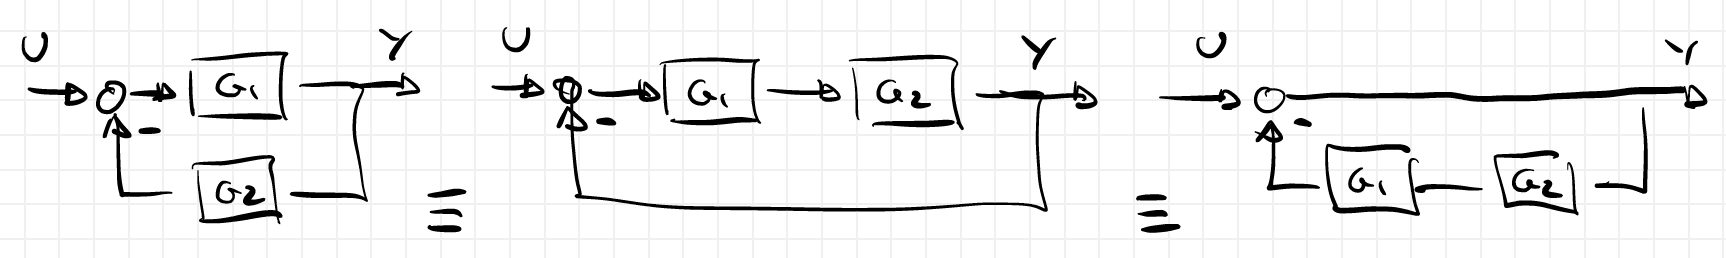
\includegraphics[width=11cm]{equivalenti}
		\end{center}
	\end{concetto}
	A questo punto è dunque possibile passare alla descrizione dei principali criteri che si possono utilizzare per determinare la stabilità (o meno) dei sistemi retroazionati.
	
	\subsection{Analisi dei poli}
		Il primo modo \textit{banale} per analizzare la stabilità dei sistemi retroazionati è quello di calcolare esplicitamente il denominatore della funzione di trasferimento e studiare la stabilità analizzando la posizione dei poli nel piano dei numeri complessi. 
		
		Nota la funzione d'anello $L(s) = N_l(s) / D_l(s)$ è possibile osservare che il denominatore polinomiale del sistema retroazionato vale $D_f = 1 \mp L(s) = D_l \mp N_l(s)$. Questo criterio, per quanto applicabile, risulta essere inefficace per sistemi di ordine elevato (in quanto le operazioni di somma polinomiale e fattorizzazione sono difficoltose).\\
		Questo metodo inoltre non può essere applicato a sistemi a ritardo di tempo, in quanto il denominatore di $G_l(s)$ vale $1+Le^{-\tau s}$: essendo questa trasformata non razionale, decade la possibilità di usare il metodo basato sul calcolo delle radici del denominatore.
		
	
	\subsection{Criterio di Nyquist}
		
		\begin{concetto}
			Il \textbf{criterio di Nyquist} è un metodo grafico basato sull'analisi del diagramma di Nyquist della funzione d'anello della retroazione.
		\end{concetto}
		
		\paragraph{Diagramma di Nyquist} Il diagramma di Nyquist deriva direttamente dal diagramma polare della funzione di trasferimento $G(i\omega)$ nel dominio della frequenza; in particolare il diagramma di Nyquist è la versione \textit{specchiata} rispetto all'asse reale del diagramma polare e si considera come \textit{verso di percorrenza} quello che parte da $\omega= 0$ fino a $\omega\rightarrow \infty$ (rispetto la parte polare, mentre la parte specchiata continuerà tale percorso, ossia andando da $\infty$ a 0) come in figura \ref{diag-nyquist}.
		
		\figura{7}{0.7}{diag-nyquist}{diagramma polare e relativo diagramma di Nyquist.}{diag-nyquist}
		
		\begin{teorema}{criterio di Nyquist per l'asintotica stabilità di un sistema retroazionato}
			\texttt{Ipotesi: } Questo criterio può essere applicato solamente quando il guadagno d'anello $L(s)$ non presenta parti nascoste associate alla cancellazione di parti legate a poli instabili; questo metodo può essere applicato solamente per sistemi negativamente retroazionati.
			
			\vspace{3mm}
			\texttt{Definizioni: } Si definisce con $P$ il numero di poli del guadagno d'anello $L(s)$ a parte reale positiva, mentre si definisce $N$ il numero di giri, contati positivamente in senso orario, del diagramma di Nyquist attorno al punto $-1$. Si osserva dunque che $P$ è sempre $\geq 0$, mentre $N$ può essere sia positivo che negativo.
			
			\vspace{3mm}
			\texttt{Enunciato:} {\itshape  Condizione necessaria e sufficiente di asintotica stabilità di un sistema negativamente retroazionato è che:
			\begin{itemize}
				\item il numero $N$ di giri intorno al punto $-1$ sia "ben definito", ossia che il diagramma di Nyquist non passi esplicitamente per tale punto;
				\item che $N$ sia uguale a $P$.
		\end{itemize}}
		\end{teorema}
		
		
		
		
	
	
	
	
	
	